\section{Setup}

\section{Single flow overhead}

\textbf{Throughput}

\begin{figure}
    \centering
    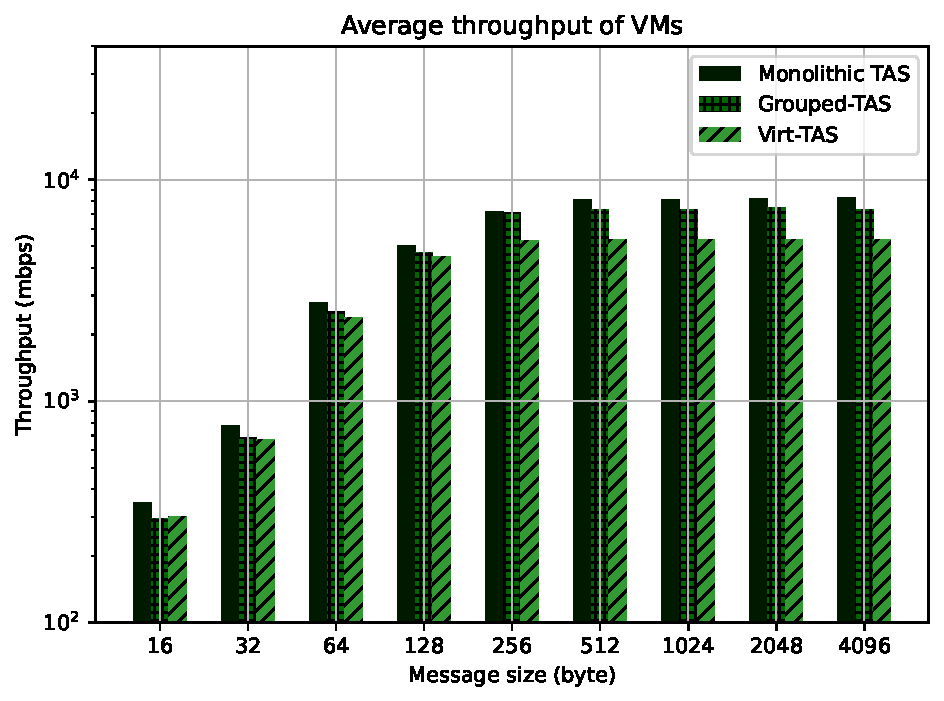
\includegraphics[scale=0.8]{../results/overhead.throughput.pdf}
    \caption{Single context overhead.}
    \label{fig:overhead.throughput}
\end{figure}

\textbf{Latency}





\section{Multiplexing}
By using a shared TCP fast-path among multiple virtual machines, tenants would benefit from the 
multiplexing benefits. To 

\begin{figure}
    \centering
    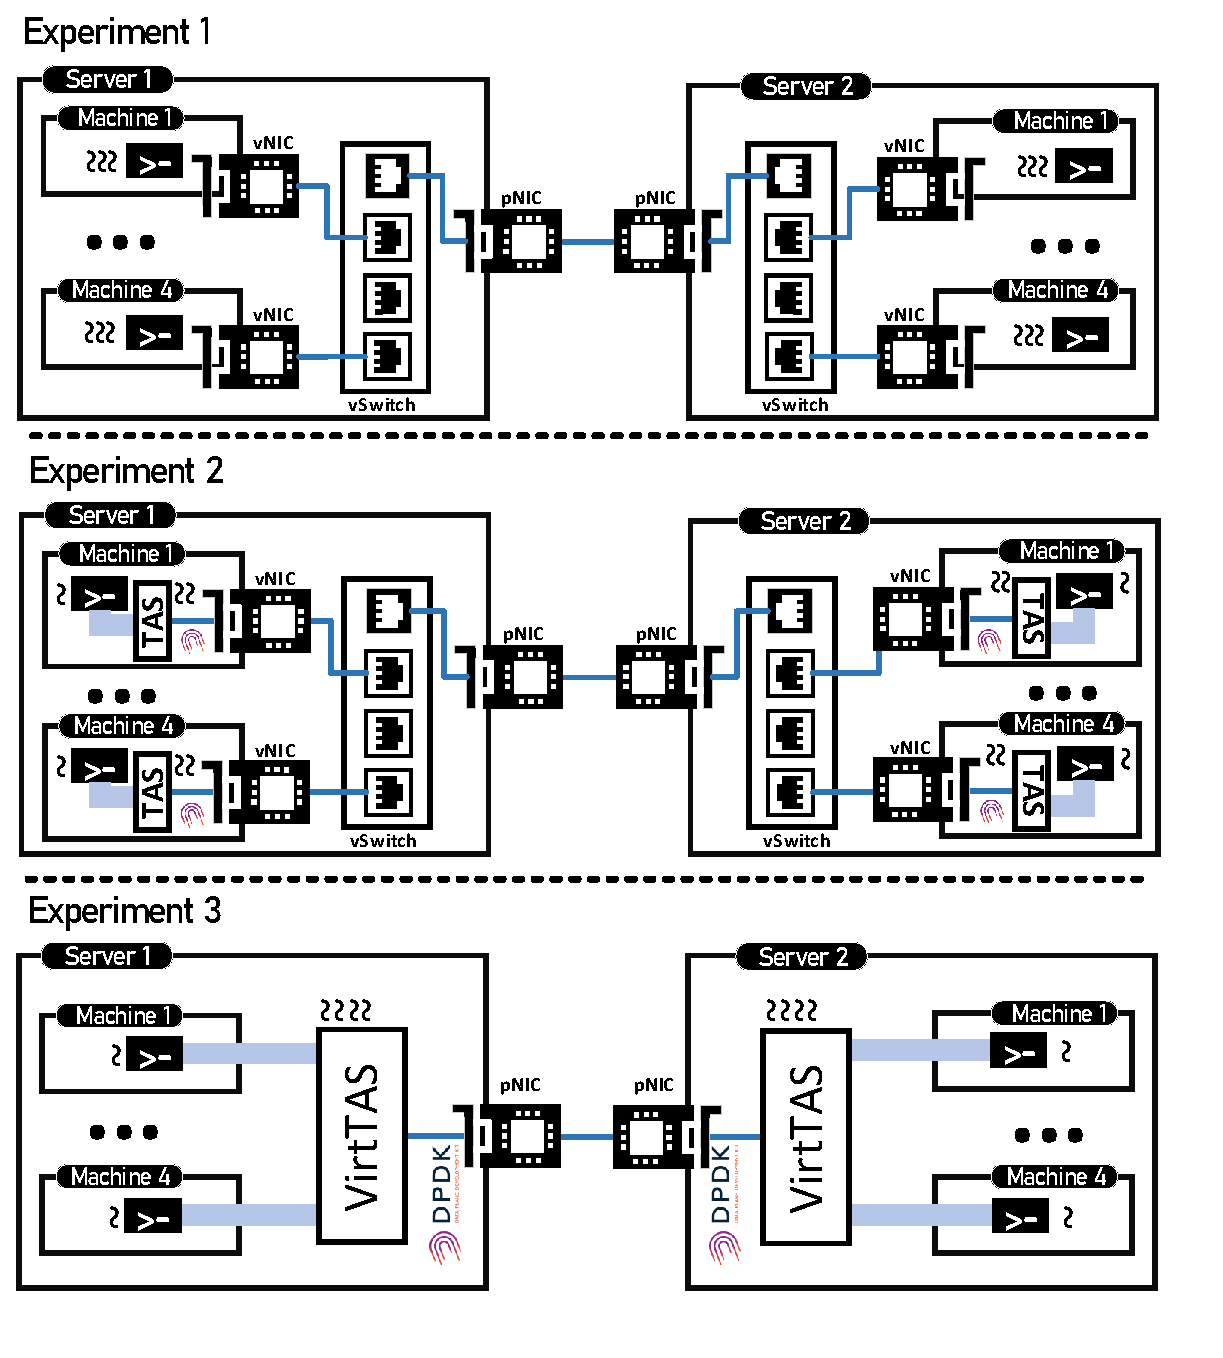
\includegraphics[scale=0.75]{../Figures/multiplexing.experiment.pdf}
    \caption{Multiplexing experiment setup.}
    \label{fig:multiplexing.experiment}
\end{figure}

\begin{figure}
    \centering
    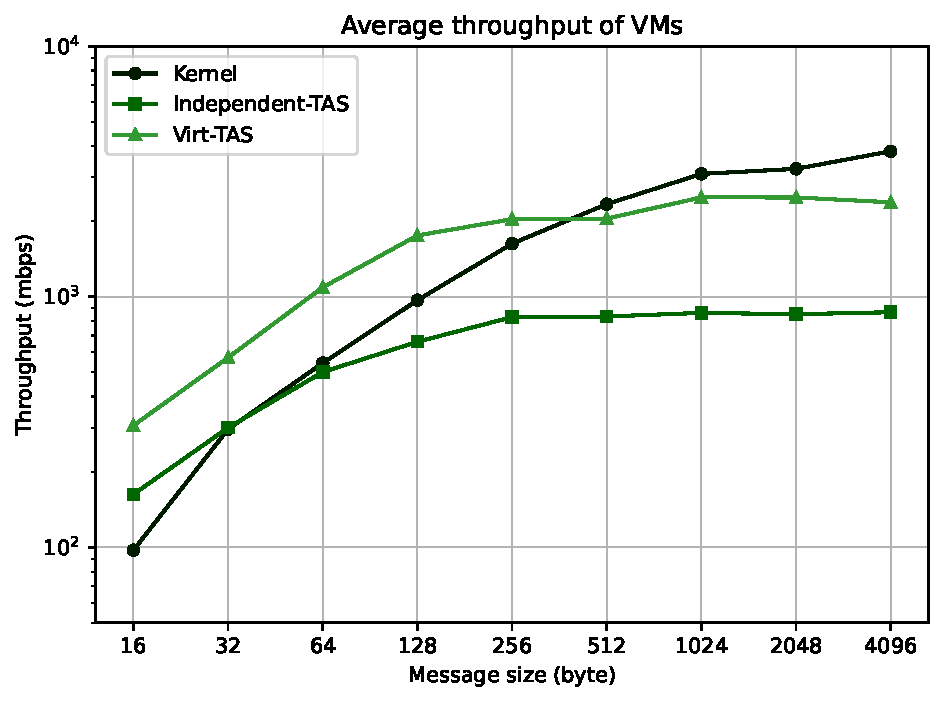
\includegraphics[scale=0.8]{../results/multiplex.throughput.pdf}
    \caption{Using a shared TCP fast-path increase the resource efficiency in  a multi-tenant environment}
    \label{fig:multiplex.throughput}
\end{figure}



\section{Flow scaling}